\chapter{Monte Carlo Simulation}    

The modern version of the Monte Carlo method was invented in the late
1940s by Stanislaw Ulam, while he was working on nuclear weapons
projects at the Los Alamos National Laboratory.
Monte Carlo methods, or Monte Carlo experiments, are a broad class of
computational algorithms that rely on repeated random sampling to obtain
numerical results. 
Monte Carlo simulation is widely used in many fields: engineering,
physics, computational biology, computer graphics, applied statistics,
artificial intelligence for games, search and rescue and of course
finance and business.
In this chapter we will review it and see some useful application to finance.

\section{The algorithm}\label{whats-monte-carlo-simulation}

The underlying concept to Monte Carlo simulation is to use randomness to solve
problems that might be deterministic in principle. These methods
are mainly used in three problem classes: optimisation, numerical
integration, and generating draws from a probability distribution.

In principle, Monte Carlo can be used to solve any problem
having a probabilistic interpretation since by the law of large numbers, the
expected value of some random variable can be approximated by taking the
empirical mean of independent samples of the variable.

Monte Carlo methods vary, but tend to follow this particular pattern:

\begin{itemize}
\tightlist
\item
  define a domain of possible inputs;
\item
  generate inputs randomly from a probability distribution over the
  defined domain;
\item
  perform a deterministic computation on the generated inputs;
\item
  aggregate the results.
\end{itemize}

\section{Pseudo-Random Numbers}\label{pseudo-random-numbers}

Uses of Monte Carlo methods require large amounts of random numbers to
generate the inputs, and it was their use that spurred the development
of pseudorandom number generators. 

Every language has libraries that
allows to produce huge series of random numbers (with a periodicity of
\(2^{19937}\)). Those numbers are produced by algorithms that take as
input a \emph{seed} which determines univokely the series. This means
that setting the same seed you will produce the same set of numbers
every time (which is great for debugging purpouses).

In \texttt{python} the right module to use is \texttt{random} which has the
following useful functions:

\begin{itemize}
\tightlist
\item
  \texttt{seed} set the seed of the random number generator;
\item
  \texttt{random} returns a random number between 0 and 1 (with uniform
  probability);
\item
  \texttt{randint(min,\ max)} returns an integer random number between
  \texttt{min} and \texttt{max} (with uniform probability);
\item
  \texttt{sample(aList,\ k=n)} samples n elements from the list
  \texttt{aList}.
\end{itemize}

As usual for a more detailed description check \texttt{help(random)}.

\begin{tcolorbox}[breakable, size=fbox, boxrule=1pt, pad at break*=1mm,colback=cellbackground, colframe=cellborder]
\begin{Verbatim}[commandchars=\\\{\}]
\PY{k+kn}{import} \PY{n+nn}{random} 

\PY{n}{random}\PY{o}{.}\PY{n}{seed}\PY{p}{(}\PY{l+m+mi}{1}\PY{p}{)}
\PY{n+nb}{print} \PY{p}{(}\PY{l+s+s2}{\PYZdq{}}\PY{l+s+s2}{seed is 1}\PY{l+s+s2}{\PYZdq{}}\PY{p}{)}
\PY{n+nb}{print}\PY{p}{(}\PY{n}{random}\PY{o}{.}\PY{n}{random}\PY{p}{(}\PY{p}{)}\PY{p}{)}
\PY{n+nb}{print}\PY{p}{(}\PY{n}{random}\PY{o}{.}\PY{n}{random}\PY{p}{(}\PY{p}{)}\PY{p}{)}

\PY{n}{random}\PY{o}{.}\PY{n}{seed}\PY{p}{(}\PY{l+m+mi}{2}\PY{p}{)}
\PY{n+nb}{print} \PY{p}{(}\PY{l+s+s2}{\PYZdq{}}\PY{l+s+s2}{seed is 2}\PY{l+s+s2}{\PYZdq{}}\PY{p}{)}
\PY{n+nb}{print}\PY{p}{(}\PY{n}{random}\PY{o}{.}\PY{n}{random}\PY{p}{(}\PY{p}{)}\PY{p}{)}
\PY{n+nb}{print}\PY{p}{(}\PY{n}{random}\PY{o}{.}\PY{n}{random}\PY{p}{(}\PY{p}{)}\PY{p}{)}

\PY{n}{random}\PY{o}{.}\PY{n}{seed}\PY{p}{(}\PY{l+m+mi}{1}\PY{p}{)}
\PY{n+nb}{print} \PY{p}{(}\PY{l+s+s2}{\PYZdq{}}\PY{l+s+s2}{seed is 1 again}\PY{l+s+s2}{\PYZdq{}}\PY{p}{)}
\PY{n+nb}{print}\PY{p}{(}\PY{n}{random}\PY{o}{.}\PY{n}{random}\PY{p}{(}\PY{p}{)}\PY{p}{)}
\PY{n+nb}{print}\PY{p}{(}\PY{n}{random}\PY{o}{.}\PY{n}{random}\PY{p}{(}\PY{p}{)}\PY{p}{)}

\PY{n+nb}{print}\PY{p}{(}\PY{n}{random}\PY{o}{.}\PY{n}{randint}\PY{p}{(}\PY{l+m+mi}{1}\PY{p}{,} \PY{l+m+mi}{10}\PY{p}{)}\PY{p}{)}
\PY{n}{aList} \PY{o}{=} \PY{p}{[}\PY{l+s+s1}{\PYZsq{}}\PY{l+s+s1}{a}\PY{l+s+s1}{\PYZsq{}}\PY{p}{,} \PY{l+s+s1}{\PYZsq{}}\PY{l+s+s1}{b}\PY{l+s+s1}{\PYZsq{}}\PY{p}{,} \PY{l+s+s1}{\PYZsq{}}\PY{l+s+s1}{c}\PY{l+s+s1}{\PYZsq{}}\PY{p}{,} \PY{l+s+s1}{\PYZsq{}}\PY{l+s+s1}{d}\PY{l+s+s1}{\PYZsq{}}\PY{p}{,} \PY{l+s+s1}{\PYZsq{}}\PY{l+s+s1}{f}\PY{l+s+s1}{\PYZsq{}}\PY{p}{]}
\PY{n+nb}{print} \PY{p}{(}\PY{n}{random}\PY{o}{.}\PY{n}{sample}\PY{p}{(}\PY{n}{aList}\PY{p}{,} \PY{n}{k}\PY{o}{=}\PY{l+m+mi}{2}\PY{p}{)}\PY{p}{)}

seed is 1
0.13436424411240122
0.8474337369372327
seed is 2
0.9560342718892494
0.9478274870593494
seed is 1 again
0.13436424411240122
0.8474337369372327
2
['c', 'a']
    \end{Verbatim}
\end{tcolorbox}

Below an example of how it can be drawn a uniform distribution.

 \begin{tcolorbox}[breakable, size=fbox, boxrule=1pt, pad at break*=1mm,colback=cellbackground, colframe=cellborder]
\begin{Verbatim}[commandchars=\\\{\}]
\PY{n}{numbers} \PY{o}{=} \PY{p}{[}\PY{p}{]}
\PY{k}{for} \PY{n}{\PYZus{}} \PY{o+ow}{in} \PY{n+nb}{range}\PY{p}{(}\PY{l+m+mi}{10000}\PY{p}{)}\PY{p}{:}
  \PY{n}{numbers}\PY{o}{.}\PY{n}{append}\PY{p}{(}\PY{n}{random}\PY{o}{.}\PY{n}{randint}\PY{p}{(}\PY{l+m+mi}{0}\PY{p}{,} \PY{l+m+mi}{5}\PY{p}{)}\PY{p}{)}

\PY{k+kn}{from} \PY{n+nn}{matplotlib} \PY{k}{import} \PY{n}{pyplot} \PY{k}{as} \PY{n}{plt}
\PY{n}{plt}\PY{o}{.}\PY{n}{hist}\PY{p}{(}\PY{n}{numbers}\PY{p}{,} \PY{l+m+mi}{6}\PY{p}{,} \PY{n+nb}{range}\PY{o}{=}\PY{p}{[}\PY{o}{\PYZhy{}}\PY{l+m+mf}{0.5}\PY{p}{,} \PY{l+m+mf}{5.5}\PY{p}{]}\PY{p}{)}
\PY{n}{plt}\PY{o}{.}\PY{n}{title}\PY{p}{(}\PY{l+s+s2}{\PYZdq{}}\PY{l+s+s2}{Uniform distribution from randint}\PY{l+s+s2}{\PYZdq{}}\PY{p}{)}
\PY{n}{plt}\PY{o}{.}\PY{n}{show}\PY{p}{(}\PY{p}{)}
\end{Verbatim}
\end{tcolorbox}

    \begin{center}
    \adjustimage{max size={0.9\linewidth}{0.9\paperheight}}{lecture_6_files/lecture_6_28_0.png}
    \end{center}
    { \hspace*{\fill} \\}
    
Another useful module that we will use later is \texttt{numpy}, it has similar functionalities as \texttt{random} but in 
some cases it can fit better to our needs.    

Below an example with \texttt{numpy.random} which allows
to throw random numbers according to a normal distribution
(\(\mathcal{N}(0, 1)\)).

    \begin{tcolorbox}[breakable, size=fbox, boxrule=1pt, pad at break*=1mm,colback=cellbackground, colframe=cellborder]
\begin{Verbatim}[commandchars=\\\{\}]
\PY{k+kn}{from} \PY{n+nn}{numpy}\PY{n+nn}{.}\PY{n+nn}{random} \PY{k}{import} \PY{n}{normal}
\PY{k+kn}{from} \PY{n+nn}{matplotlib} \PY{k}{import} \PY{n}{pyplot} \PY{k}{as} \PY{n}{plt}

\PY{n}{gauss} \PY{o}{=} \PY{p}{[}\PY{p}{]}
\PY{k}{for} \PY{n}{\PYZus{}} \PY{o+ow}{in} \PY{n+nb}{range}\PY{p}{(}\PY{l+m+mi}{50000}\PY{p}{)}\PY{p}{:}
  \PY{n}{gauss}\PY{o}{.}\PY{n}{append}\PY{p}{(}\PY{n}{normal}\PY{p}{(}\PY{p}{)}\PY{p}{)}
  
\PY{n}{plt}\PY{o}{.}\PY{n}{hist}\PY{p}{(}\PY{n}{gauss}\PY{p}{,} \PY{l+m+mi}{100}\PY{p}{,} \PY{n+nb}{range}\PY{o}{=}\PY{p}{[}\PY{o}{\PYZhy{}}\PY{l+m+mi}{4}\PY{p}{,} \PY{l+m+mi}{4}\PY{p}{]}\PY{p}{)}
\PY{n}{plt}\PY{o}{.}\PY{n}{title}\PY{p}{(}\PY{l+s+s2}{\PYZdq{}}\PY{l+s+s2}{Example of gaussian distribution from numpy}\PY{l+s+s2}{\PYZdq{}}\PY{p}{)}
\PY{n}{plt}\PY{o}{.}\PY{n}{show}\PY{p}{(}\PY{p}{)}
\end{Verbatim}
\end{tcolorbox}

    \begin{center}
    \adjustimage{max size={0.9\linewidth}{0.9\paperheight}}{lecture_6_files/lecture_6_32_0.png}
    \end{center}
    { \hspace*{\fill} \\}

    
\section{Practical Examples of Monte Carlo
Simulation}\label{example-of-monte-carlo-simulation}

In this section we go through some simple applications of the method .

\subsubsection{Probability to draw two kings from a deck}
Using a frequentist approach, we can calculate the
probability of an event as the ratio of the number of favourable outcomes
of an experiment (number of successes) and the number of all possible
outcomes so for our example.

At the beginning we have 40 cards (i.e. the entire deck) with 4 kings so the probability to get a king
is $4/40$. Next, assuming we got a king the first time, we are left with 39 cards and 3 kings only so the 
probability to get the second king is $3/39$. Since the two draws are independent, the total probability 
is product of the two contributions, indeed:

\[P_\textrm{two kings} = \frac{4}{40} \cdot \frac{3}{39} = \frac{1}{130} \approx 0.0077\]

Let's now try with a Monte Carlo simulation following the steps outlined above.
Define a domain of possible inputs: in this case the domain is a deck of cards. With the \texttt{*} operator a list can be easily repeated many times.
In this case we do it 4 times, once for the different suits.

\begin{tcolorbox}[breakable, size=fbox, boxrule=1pt, pad at break*=1mm,colback=cellbackground, colframe=cellborder]
\begin{Verbatim}[commandchars=\\\{\}]
\PY{k+kn}{from} \PY{n+nn}{random} \PY{k}{import} \PY{n}{sample}\PY{p}{,} \PY{n}{choices}\PY{p}{,} \PY{n}{seed}

\PY{n}{seed}\PY{p}{(}\PY{l+m+mi}{1}\PY{p}{)}

\PY{n}{deck} \PY{o}{=} \PY{p}{[}\PY{l+s+s2}{\PYZdq{}}\PY{l+s+s2}{A}\PY{l+s+s2}{\PYZdq{}}\PY{p}{,} \PY{l+s+s2}{\PYZdq{}}\PY{l+s+s2}{2}\PY{l+s+s2}{\PYZdq{}}\PY{p}{,} \PY{l+s+s2}{\PYZdq{}}\PY{l+s+s2}{3}\PY{l+s+s2}{\PYZdq{}}\PY{p}{,} \PY{l+s+s2}{\PYZdq{}}\PY{l+s+s2}{4}\PY{l+s+s2}{\PYZdq{}}\PY{p}{,} \PY{l+s+s2}{\PYZdq{}}\PY{l+s+s2}{5}\PY{l+s+s2}{\PYZdq{}}\PY{p}{,} \PY{l+s+s2}{\PYZdq{}}\PY{l+s+s2}{6}\PY{l+s+s2}{\PYZdq{}}\PY{p}{,} \PY{l+s+s2}{\PYZdq{}}\PY{l+s+s2}{7}\PY{l+s+s2}{\PYZdq{}}\PY{p}{,} \PY{l+s+s2}{\PYZdq{}}\PY{l+s+s2}{J}\PY{l+s+s2}{\PYZdq{}}\PY{p}{,} \PY{l+s+s2}{\PYZdq{}}\PY{l+s+s2}{Q}\PY{l+s+s2}{\PYZdq{}}\PY{p}{,} \PY{l+s+s2}{\PYZdq{}}\PY{l+s+s2}{K}\PY{l+s+s2}{\PYZdq{}}\PY{p}{]} \PY{o}{*} \PY{l+m+mi}{4}
 \end{Verbatim}
\end{tcolorbox}

Next, we generate inputs randomly from a probability distribution over the defined domain: which means we draw randomly cards
with uniform probability since the deck is fair and all cards have the same probability to be drawn. 
We plan to do 1 million of simulations (our denominator), each time with the \texttt{sample} function we pick up two cards from our virtual deck with 
uniform probability. For debugging purpouse the first 10 trials are printed.

\begin{tcolorbox}[breakable, size=fbox, boxrule=1pt, pad at break*=1mm,colback=cellbackground, colframe=cellborder]
\begin{Verbatim}[commandchars=\\\{\}]
\PY{n}{trials} \PY{o}{=} \PY{l+m+mi}{1000000}
\PY{n}{success} \PY{o}{=} \PY{l+m+mi}{0}

\PY{k}{for} \PY{n}{i} \PY{o+ow}{in} \PY{n+nb}{range}\PY{p}{(}\PY{n}{trials}\PY{p}{)}\PY{p}{:}
  \PY{n}{cards} \PY{o}{=} \PY{n}{sample}\PY{p}{(}\PY{n}{deck}\PY{p}{,} \PY{n}{k}\PY{o}{=}\PY{l+m+mi}{2}\PY{p}{)}
  \PY{k}{if} \PY{n}{i} \PY{o}{\PYZlt{}} \PY{l+m+mi}{10}\PY{p}{:}
    \PY{n+nb}{print} \PY{p}{(}\PY{n}{cards}\PY{p}{)}
\end{Verbatim}
\end{tcolorbox}

Perform a deterministic computation on the generated inputs: this step is particularly simple in this case, we just need to check if the draw
is \texttt{['K', 'K']} and in case increase the counter of successes.

\begin{tcolorbox}[breakable, size=fbox, boxrule=1pt, pad at break*=1mm,colback=cellbackground, colframe=cellborder]
\begin{Verbatim}[commandchars=\\\{\}]
  \PY{k}{if} \PY{n}{cards} \PY{o}{==} \PY{p}{[}\PY{l+s+s2}{\PYZdq{}}\PY{l+s+s2}{K}\PY{l+s+s2}{\PYZdq{}}\PY{p}{,} \PY{l+s+s2}{\PYZdq{}}\PY{l+s+s2}{K}\PY{l+s+s2}{\PYZdq{}}\PY{p}{]}\PY{p}{:}
    \PY{n}{success} \PY{o}{+}\PY{o}{=} \PY{l+m+mi}{1}
 \end{Verbatim}
\end{tcolorbox}

Aggregate the results: finally we just print success/trials which is the sought probability.

\begin{tcolorbox}[breakable, size=fbox, boxrule=1pt, pad at break*=1mm,colback=cellbackground, colframe=cellborder]
\begin{Verbatim}[commandchars=\\\{\}]
\PY{n+nb}{print} \PY{p}{(}\PY{l+s+s2}{\PYZdq{}}\PY{l+s+s2}{The probability to draw two kings is }\PY{l+s+si}{\PYZob{}:.4f\PYZcb{}}\PY{l+s+s2}{\PYZdq{}}\PY{o}{.}\PY{n}{format}\PY{p}{(}\PY{n}{success}\PY{o}{/}\PY{n}{trials}\PY{p}{)}\PY{p}{)}

['Q', '7']
['5', '7']
['J', '2']
['Q', 'A']
['5', '4']
['7', '2']
['2', '5']
['J', 'Q']
['A', 'Q']
['J', '5']
The probability to draw two kings is 0.0077
    \end{Verbatim}
\end{tcolorbox}

\subsubsection{Dice probabilities}
Two dice are rolled, find the probability that the sum is:
\begin{enumerate}
\item equal to 1
\item equal to 4
\item less than 13
\end{enumerate}

Before looking at the \texttt{python} implementation let's compute what we should get: the possible combinations
of the outcomes of two dice are 36 (to realize it you can simply write down them). It is not possible to get 1 since
thee dice have no face with 0 so the first probability should come 0. The sum of the two dice is always less then 13 
(the maximum is 12...) so the answer to point 3 is 1. We can get a sum of 4 in 3 cases (1-3, 3-1 or 2-2) so the 
probaiblity will result $3/36=1/12=0.0833$


%%%%%%%%%%%%%%%%%%%%%%%%%%%%%%%%%%%

Since we rely on a frequentist approach the lower is the probability we need to estimate the higher has to be the number
of simulated trials. This is because to get a reasonable number of "success" in order to get a low uncertainty in the probability
we have to try many times. This is apparent playing with the number of trials in the above simulations.

 \subsection{Derivation of log-normal Stochastic Differential
Equation}\label{derivation-of-log-normal-stochastic-differential-equation}

Stock prices deviate from a steady state as a result of the random
fluctuations given by the trades. Considering a stock with a price
\(S_t\) and an expected rate of return \(\mu\), then the relative change
in its price during a period \(dt\) can be decomposed in two parts:

\begin{itemize}
\tightlist
\item
  a deterministic part that is the expected return from the stock held
  during the time period \(dt\) (\(\mu S_tdt\))
\item
  a stochastic part which reflects the random changes of the market
  (e.g.~as a response to external effects such as unexpected news). A
  reasonable assumption is to take this contribution proportional to the
  stock (\(\sigma S_tdB_t\) where \(dB_t\) is a random walk process
  equal to \(\mathcal{N}(0,1)\sqrt{t}\)).
\end{itemize}

    The resulting differential equation is:

\[dS_t = \mu S_tdt + \sigma S_tdB_t\] or
\[\frac{dS_t}{S_t} = d\textrm{log}(S_t) = \mu dt + \sigma dB_t\]

    The solution of this equation can be derived by applying the
It\(\hat{o}\)'s formula which states that for any given function
\(G(S, t)\) where \(S\) satisfies the following stochastic differential
equation \(dS=a\cdot dt +b\cdot dB_t\) it holds:

\[dG=\big(a\frac{\partial G}{\partial S} + \frac{\partial G}{\partial t} + \frac{1}{2}b^2\frac{\partial^2 G}{\partial S^2} \big)dt + b \frac{\partial G}{\partial S}dB\]

Considering \(G = \textrm{log}(S_t)\) we have:

\[\frac{\partial G}{\partial S} = \frac{1}{S_t}\]

\[\frac{\partial G}{\partial t} = 0\]

\[\frac{\partial^2 G}{\partial S^2} = -\frac{1}{S_t^{2}}\]

    By inserting these into It\(\hat{o}\)'s formula we get:

\[d(\textrm{log} S_t) = \big(\mu S_t \frac{1}{S_t} + \frac{1}{2}\sigma^2 S_t^2 (-\frac{1}{S_t^2})\big)dt + \sigma\epsilon\sqrt{dt}\]

\[d(\textrm{log} S_t) = \textrm{log} (S_t) - \textrm{log} (S_{t-1}) = \textrm{log} \frac{S_t}{S_{t-1}} = \big(\mu - \frac{1}{2}\sigma^2\big)dt + \sigma\epsilon\sqrt{dt}\]

\[S_t = S_{t-1}e^{\big(\mu - \frac{1}{2}\sigma^2\big)dt + \sigma\epsilon\sqrt{dt}}\]

    As can be seen from the following equation:

\[d(\textrm{log} S_t) = \big(\mu - \frac{1}{2}\sigma^2\big)dt + \sigma\epsilon\sqrt{dt}\]
the change in \(\textrm{log} S_t\) has a constant \emph{drift}
\(\mu - \frac{1}{2}\sigma^2\) and a constance variance rate \(\sigma^2\)
(remember that \(\epsilon\) is a normally distributed random variable
(\(\mathcal{N}(0,1)\)). So you have a constant plus a gaussian
distributed variable, therefore \(\textrm{log} S_t\) at some time \(T\)
is normally distributed with:

\[\textrm{log}S_t - \textrm{log}S_0 \approx\mathcal{N}\big[\big(\mu-\frac{\sigma^2}{2}\big)T, \sigma^2 T\big]\]

This equation shows that \(\textrm{log}S_t\) is normally distributed,
but \textbf{a variable whose logarithm is normally distributed is said
to be log-normal}. Hence the model we have just developed implies that
the stock price at time T, given today's price, is lognormally
distributed. One of the nicer property of a log-normal distribution is to be positive defined 
and that's why lognormality is important because we need to ensure that a stock price
will never be negative. Indeed looking at the initial \(dS\) equation we
have that:

\[dS_t = \mu S_tdt + \sigma S_tdB_t\]
which shows that the closer is \(S_t\) to 0 the smaller is the \(dS\)
variation (so it will never go below 0).

The previous calculation will be useful to simulate the course of a stock price for example.

\subsection{Confidence interval}\label{confidence-interval}

Whenever a quantity is determined with a Monte Carlo simulation the confidence interval
concept comes in hand, indeed it helps to assess how good is our estimate.

X\% confidence interval can be interpreted by saying that there is X\%
probability that the calculated interval from another (different)
simulation contains the true value of the estimated parameter. In other
words X\% confidence interval can be expressed in terms of repeated
experiments (or samples) like the following: if you repeat many time the above simulation,
hence \(\mathcal{N}\) is sampled many times, the fraction of calculated
confidence intervals (which would differ for each sample) that contains
the true parameter would tend toward X\%

\begin{figure}[h]
\centering
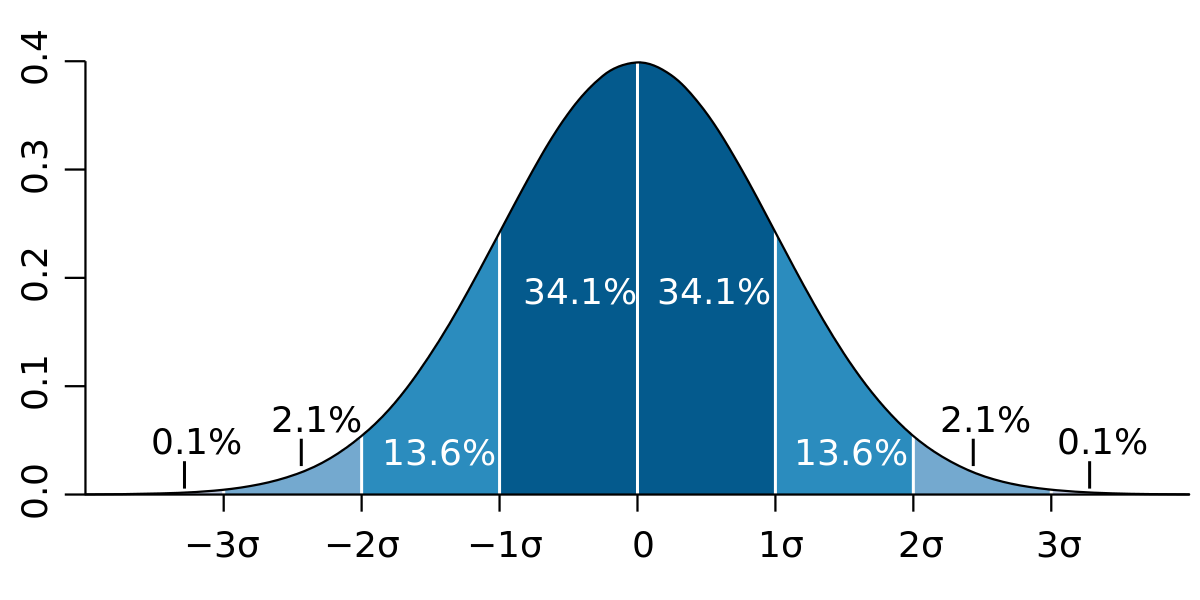
\includegraphics{Standard_deviation_diagram.svg.png}
\caption{Confidence interval graphical explanation}
\end{figure}

A Confidence Interval is a range of values we are fairly sure our true value lies in.

men running
Example: Average Height
We measure the heights of 40 randomly chosen men, and get a mean height of 175cm,

We also know the standard deviation of men's heights is 20cm.

The 95% Confidence Interval (we show how to calculate it later) is:

175cm � 6.2cm

confidence interval 175 plus minus 6.2

This says the true mean of ALL men (if we could measure all their heights) is likely to be between 168.8cm and 181.2cm.

But it might not be!

The "95%" says that 95% of experiments like we just did will include the true mean, but 5% won't.

So there is a 1-in-20 chance (5%) that our Confidence Interval does NOT include the true mean.





Step 1: start with

the number of observations n
the mean X
and the standard deviation s
Note: we should use the standard deviation of the entire population, but in many cases we won't know it.

We can use the standard deviation for the sample if we have enough observations (at least n=30, hopefully more).

Using our example:

number of observations n = 40
mean X = 175
standard deviation s = 20
Step 2: decide what Confidence Interval we want: 95% or 99% are common choices. Then find the "Z" value for that Confidence Interval here:

Confidence
Interval	Z
80%	1.282
85%	1.440
90%	1.645
95%	1.960
99%	2.576
99.5%	2.807
99.9%	3.291
For 95% the Z value is 1.960

Step 3: use that Z value in this formula for the Confidence Interval

X  �  Z s�n 

Where:

X is the mean
Z is the chosen Z-value from the table above
s is the standard deviation
n is the number of observations
And we have:

175 � 1.960 ?  20�40 

Which is:

175cm � 6.20cm

In other words: from 168.8cm to 181.2cm


Also from here is clear that increasing the number of experiments the confidence interval becomes narrower hence
how estimate is more precise.
 